\chapter{费米子质量：手征性、汤川耦合与马约拉纳中微子}

\lectureoverview{我们首先在一个玩具\(U(1)\)理论中重建规范玻色子希格斯机制，然后对费米子提出平行的问题。狄拉克质量混合左手与右手手征场，但弱相互作用赋予它们不同的电荷，因此禁止裸质量。与希格斯场的汤川耦合尊重该对称性；在希格斯场获得真空值之后，同一相互作用变成费米子质量和可测量的希格斯--费米子耦合。最后一部分沿着这一逻辑进入中微子质量、可能的无保护重粒子、宇宙线运动学、相对论惯性和引力。}

开场回顾的目的不仅仅是重复上一讲。我们需要从中提取一个可以搬到费米子上的想法：质量是零动量激发态的非零能量。对于场而言，零动量意味着无限波长，或者说处处相同的位移。仅含导数的理论无法探测均匀位移。不含导数的项则可以。

\section{规范玻色子故事一遍过}

\subsection{导数能量与无质量矢量}

模型规范场是\(A_\mu\)，场强为
\begin{equation}
  F_{\mu\nu}
  =\partial_\mu A_\nu-\partial_\nu A_\mu .
  \label{eq:l09-field-strength}
\end{equation}
黑板上把规范动能项示意性地写成\(F^2\)。在标准归一化下它是
\begin{equation}
  \mathcal L_{\mathrm{gauge}}
  =-\frac14 F_{\mu\nu}F^{\mu\nu}.
  \label{eq:l09-gauge-kinetic}
\end{equation}

\begin{figure}[htbp]
\centering
\includegraphics[width=0.72\textwidth]{lecture_09_figure_02.png}
\caption{场强定义以及黑板上用于规范场导数能量的\(F^2\)简写。}
\lectureframe{00:02:39}
\label{fig:l09-field-strength-board}
\end{figure}

\eqref{eq:l09-gauge-kinetic}中每一次出现\(A_\mu\)都被求导。因此，
\begin{equation}
  A_\mu(x)\longmapsto A_\mu(x)+c_\mu,
  \qquad \partial_\nu c_\mu=0,
\end{equation}
不改变\(F_{\mu\nu}\)。所以均匀的矢量势不消耗任何场强能量。用本讲的语言说，零动量模没有能隙，规范玻色子是无质量的。

这个\(U(1)\)场是一个刻意简化的替身。物理目标是\(W^\pm\)和\(Z\)，而不是电磁光子。未破缺的电磁对称性使光子保持无质量；破缺的电弱对称性赋予弱规范玻色子质量。

\subsection{冻结希格斯半径}

引入一个带电复标量场，并将其写成极坐标形式，
\begin{equation}
  \phi(x)=\rho(x)e^{i\alpha(x)}.
\end{equation}
它的墨西哥帽势在非零半径的圆上取极小值。称该半径为\(f\)，径向方向相对较硬。第一遍我们先把它冻结，只保留相位：
\begin{equation}
  \phi(x)\simeq f e^{i\alpha(x)}.
  \label{eq:l09-frozen-higgs}
\end{equation}

\begin{figure}[htbp]
\centering
\includegraphics[width=0.72\textwidth]{lecture_09_figure_03.png}
\caption{冻结的希格斯半径、其协变导数，以及回顾中使用的小型破缺势草图。}
\lectureframe{00:06:42}
\label{fig:l09-frozen-board}
\end{figure}

选择约定
\begin{equation}
\begin{aligned}
  D_\mu&=\partial_\mu+igA_\mu,
  \\
  \phi&\longmapsto e^{i\theta}\phi,
  \\
  A_\mu&\longmapsto A_\mu-\frac1g\partial_\mu\theta .
\end{aligned}
  \label{eq:l09-gauge-convention}
\end{equation}
本讲将\(g\)省略；让它显式出现可以使量纲和最终质量变得透明。作用在冻结场上给出
\begin{align}
  D_\mu\phi
  &=(\partial_\mu+igA_\mu)f e^{i\alpha}
  \notag\\
  &=i\bigl(\partial_\mu\alpha+gA_\mu\bigr)
    f e^{i\alpha}.
  \label{eq:l09-covariant-frozen}
\end{align}
乘以复共轭消去相位，并且把\(i\)乘以\(-i\)变成\(+1\)：
\begin{equation}
  |D_\mu\phi|^2
  =f^2
   \bigl(\partial_\mu\alpha+gA_\mu\bigr)
   \bigl(\partial^\mu\alpha+gA^\mu\bigr).
  \label{eq:l09-frozen-square}
\end{equation}

\begin{classroomqa}
\audiencequestion{协变导数的平方是否应该带一个负号，因为导数产生了一个\(i\)因子？
\lecturetimestamp{00:07:39}}
\lecturerresponse{不。动能项是与复共轭的乘积。一个因子贡献\(i\)，另一个贡献\(-i\)，而\(i(-i)=1\)。\(D_\mu\)的符号约定可以一致地反转，但在相应的能量表达式中模方是正的。}
\end{classroomqa}

\eqref{eq:l09-frozen-square}中的组合本身就是一个平移后的规范场。选择\(\theta=-\alpha\)，使标量相位消失，并定义
\begin{equation}
  A'_\mu=A_\mu+\frac1g\partial_\mu\alpha .
  \label{eq:l09-unitary-gauge-field}
\end{equation}
于是
\begin{equation}
  |D_\mu\phi|^2=g^2f^2 A'_\mu A'^\mu .
  \label{eq:l09-vector-mass-term}
\end{equation}
新项不含\(A'_\mu\)的导数。均匀场现在储存能量，因此零动量矢量模有能隙。

\begin{figure}[htbp]
\centering
\includegraphics[width=0.72\textwidth]{lecture_09_figure_04.png}
\caption{黑板分离出在相位被吸收后标志规范玻色子质量的\(f^2A^2\)项。}
\lectureframe{00:10:31}
\label{fig:l09-vector-mass-board}
\end{figure}

在正则标量归一化下，人们写出
\(\phi=(f+h)e^{i\pi/f}/\sqrt2\)。将所得的矢量项与
\(\tfrac12m_A^2A_\mu A^\mu\)比较，得到
\begin{equation}
  m_A=gf
  \label{eq:l09-abelian-vector-mass}
\end{equation}
在这个阿贝尔模型中。本讲省略归一化因子，并用矢量质量由\(f\)设定来总结结果。

相位模并没有不声不响地消失。在规范化之前，它是一个无质量戈德斯通玻色子。在规范化之后，它提供了有质量矢量粒子所需的纵向极化。我们暂时冻结的径向涨落则作为物理希格斯激发保留下来。

\subsection{为什么不含导数的项意味着质量}

\begin{classroomqa}
\audiencequestion{为什么 \(A'^2\) 项算作质量，而不只是另一种相互作用？\lecturetimestamp{00:13:10}}
\lecturerresponse{质量是静止时的能量。对于场而言，静止的粒子是零动量、无限波长模式的量子。导数项不会给静态均匀位移带来能量，而 \(m_A^2A'^2\) 会。那个非零的零动量能量就是静止能量间隙。}
\end{classroomqa}

讲座通过三个力学类比来展开这一论述。

\begin{itemize}
  \item 在晶体中，缓慢变化的位移会消耗弹性势能，因为相邻原子被不同程度地移动。刚性平移使每个原子一起移动，不消耗内能。因此声学声子是能隙为零的。
  \item 在理想旋转对称磁体中，空间变化的自旋方向会消耗交换能，但将所有自旋一起旋转则不会。相关的长波长自旋波是能隙为零的。
  \item 在等离子体中，即使相对位移是均匀的，将电子流体相对于正电荷背景移动也会产生电荷分离和恢复电场。由此产生的等离激元在零波数处具有非零频率。
\end{itemize}

希格斯化后的规范场的行为类似于第三个例子：破缺的介质会抵抗原本无代价的均匀位移。

\begin{classroomqa}
\audiencequestion{在引入规范场之前，相位 \(\alpha\) 不是已经在振动了吗？\lecturetimestamp{00:18:24}}
\lecturerresponse{是的。它的能量正比于 \(f^2(\partial_\mu\alpha)^2\)。随位置变化的相位具有梯度能量，可以传播，但相位的均匀变化不消耗任何能量。这正是无质量的戈德斯通模式。}
\end{classroomqa}

\begin{classroomqa}
\audiencequestion{导数包含时间导数。实际移动整个点阵或改变整个场，难道不携带动能吗？\lecturetimestamp{00:22:18}}
\lecturerresponse{是的。比较是在静态构型之间，或在任意缓慢制备的构型之间进行的。以非零速度平移的点阵具有动能。质量检验问的是：当构型处于静止且空间均匀时，它是否仍然具有能量。}
\end{classroomqa}

\section{实验线索：弱相互作用区分左与右}

讲座现在转向电子、{\proseunicodefont μ}子和夸克。它们的质量也来自希格斯场，但机制看起来不同，因为费米子质量不是二次矢量项。它是两个手征场之间的耦合。

\subsection{{\proseunicodefont β}衰变中的宇称破缺}

从弱相互作用破坏宇称这一经验事实开始。量子电动力学和量子色动力学对某一过程及其镜像一视同仁。弱相互作用则不然。在中子{\proseunicodefont β}衰变中，\begin{equation}
  n\longrightarrow p+e^-+\bar\nu_e,
  \label{eq:l09-beta-decay}
\end{equation}
由带电流相互作用选出的高能电子具有左手螺旋度：它们的自旋指向与动量相反。相应的反中微子具有相反的螺旋度。

对于超相对论粒子，螺旋度定义为
\begin{equation}
  h=\frac{\bm S\cdot\bm p}{|\bm S|\,|\bm p|}.
\end{equation}
自旋平行于动量为 \(h=+1\)；自旋反平行于动量为 \(h=-1\)。
弱相互作用耦合到左手征电子场和左手征中微子场，而不以同样的方式耦合到右手征电子场。\editorialnote{讲座最初在螺旋度意义上使用左右手性，因为在高能下这直观可见。规范荷实际上作用于手征性，即由 \(P_L=(1-\gamma^5)/2\) 和 \(P_R=(1+\gamma^5)/2\) 选出的洛伦兹表示标签。对于无质量粒子，粒子的手征性和螺旋度一致；对于有质量粒子，它们不一致。}

为了在不使用完整的 \(SU(2)_L\times U(1)_Y\) 记账的情况下揭示这一障碍，想象一个假的 \(U(1)\) 世界，其中只有 \(\psi_L\) 携带相关荷：
\begin{equation}
  \psi_L\longmapsto e^{i\theta}\psi_L,
  \qquad
  \psi_R\longmapsto\psi_R .
  \label{eq:l09-chiral-toy-charge}
\end{equation}
这不是电磁学：真实的左手征和右手征电子携带相同的电荷。它是弱相互作用的一幅漫画，其中两种手征性处于不同的电弱表示中。

\begin{classroomqa}
\audiencequestion{同样的左--右不对称性也适用于夸克吗？\lecturetimestamp{00:31:50}}
\lecturerresponse{是的，用适当的弱多重态和超荷。左手征的上型和下型夸克组成弱二重态，而右手征场是弱单态。因此它们的希格斯耦合面临与电子相同的结构问题。}
\end{classroomqa}

\section{狄拉克质量是左--右混合}

\subsection{从四分量方程到两个韦尔方程}

狄拉克波函数有四个分量。粗略地说，其中两个描述自旋，另外两个区分正能解与负能解，而后者被重新解释为反粒子自由度。写成哈密顿形式，
\begin{equation}
  i\frac{\partial\Psi}{\partial t}
  =\left(-i\bm\alpha\cdot\bm\nabla+m\beta\right)\Psi .
  \label{eq:l09-dirac-hamiltonian}
\end{equation}
矩阵\(\alpha_i\)与\(\beta\)编码了能量、动量与质量之间的相对论关系。

\begin{figure}[htbp]
\centering
\includegraphics[width=0.74\textwidth]{lecture_09_figure_05.png}
\caption{黑板上先写出狄拉克方程，然后把它拆成相互耦合的左手方程与右手方程。}
\lectureframe{00:40:30}
\label{fig:l09-dirac-board}
\end{figure}

手征基使\(m\)的作用变得明确。取
\(\sigma^\mu=(1,\bm\sigma)\)与
\(\bar\sigma^\mu=(1,-\bm\sigma)\)，
\begin{align}
  i\bar\sigma^\mu\partial_\mu\psi_L&=m\psi_R,
  \label{eq:l09-weyl-left}\\
  i\sigma^\mu\partial_\mu\psi_R&=m\psi_L.
  \label{eq:l09-weyl-right}
\end{align}
在\(m=0\)时，两个方程彼此独立：左手征场与右手征场可以各自传播而互不交谈。在\(m\neq0\)时，二者各自成为对方的源。这正是狄拉克质量混合左右手征的确切含义。

Susskind把这一现象描述为费米子在左右之间振荡。这种说法抓住了耦合，但不应把它硬推成一个点粒子来回翻转的经典图像。精确的陈述是耦合场方程
\eqref{eq:l09-weyl-left}--\eqref{eq:l09-weyl-right}。

\begin{classroomqa}
\audiencequestion{黑板上的两个方程中，\(i\)的因子与符号是否一致？\lecturetimestamp{00:41:10}}
\lecturerresponse{逐行来看并不一致；在快速推导过程中，有一个\(i\)被不一致地提到了外面。可靠的内容是耦合模式。方程\eqref{eq:l09-weyl-left}与
\eqref{eq:l09-weyl-right}给出了一种标准且自洽的约定。}
\end{classroomqa}

\subsection{为什么弱对称性禁止裸质量}

拉格朗日量中相应的狄拉克质量项为
\begin{equation}
  \mathcal L_m
  =-m\bar\psi\psi
  =-m\left(\bar\psi_L\psi_R+\bar\psi_R\psi_L\right).
  \label{eq:l09-bare-dirac-mass}
\end{equation}
在玩具变换\eqref{eq:l09-chiral-toy-charge}下，
\begin{equation}
  \bar\psi_L\psi_R\longmapsto
  e^{-i\theta}\bar\psi_L\psi_R,
  \qquad
  \bar\psi_R\psi_L\longmapsto
  e^{i\theta}\bar\psi_R\psi_L.
\end{equation}
两项都不不变。因此，在对称性破缺之前，直接的左--右混合系数\(m\)是被禁止的。

仅凭电磁作用不会造成这个问题，因为\(\psi_L\)与
\(\psi_R\)具有相同的电荷。这一阻碍来自它们不同的弱量子数。

\subsection{暴露手征微妙之处的螺旋度问题}

课堂现在从几个角度检验直观的手性图像。这些问题并非枝节问题：它们恰好揭示了螺旋度在何处有用，以及在何处必须由手征取而代之。

\begin{classroomqa}
\audiencequestion{如果弱相互作用以相同方式发射两种电子螺旋度，世界会是什么样子？\lecturetimestamp{00:42:12}}
\lecturerresponse{在该过程中，直接的宇称不对称性会消失。但真实的电弱理论是手征的：只有左手征二重态携带带电流弱相互作用。讲座推迟了对自然界为何选择这种结构的更完整说明。}
\end{classroomqa}

\begin{classroomqa}
\audiencequestion{假设电子的自旋被制备为竖直方向，然后电子被水平加速。它是左手性的还是右手性的？\lecturetimestamp{00:42:44}}
\lecturerresponse{自旋态若横向于动量，则是两种螺旋度的叠加。只有当自旋平行或反平行于动量时，螺旋度才是确定的。尽管如此，弱手征投影算符对场仍有良好定义。}
\end{classroomqa}

有质量粒子可以被减速到静止，并沿相反方向加速，而自旋不发生反转。于是它的螺旋度改变符号。无质量粒子不能被洛伦兹助推追上或带到静止，因此它的螺旋度在固有助推下不变。这为讲座中的说法提供了动机：只有一种物理螺旋度的粒子种类必定无质量。更精确的场论陈述是，洛伦兹不变的狄拉克质量要求两种手征同时存在。

\begin{classroomqa}
\audiencequestion{圆偏振光子可以从镜面反射并反向传播，而从不静止。这是否与螺旋度论证矛盾？\lecturetimestamp{00:45:28}}
\lecturerresponse{不矛盾。镜子是一个外部系统，可以交换角动量并反转传播方向。反射过程并不是追上光子的洛伦兹助推。某个通道是否存在，还取决于允许的偏振态以及材料的边界条件。}
\end{classroomqa}

\begin{classroomqa}
\audiencequestion{普通电子束包含一种手性还是两种？\lecturetimestamp{00:46:10}}
\lecturerresponse{一般而言两种都有。有质量电子态包含两种手征分量，而非偏振束包含两种螺旋度。专门的源可以产生具有很大螺旋度不对称性的偏振束。}
\end{classroomqa}

\begin{classroomqa}
\audiencequestion{束流能否独立于其自旋被聚焦，还是磁场会将两种极化分开？\lecturetimestamp{00:46:29}}
\lecturerresponse{通常的位置聚焦可以在很大程度上对自旋不敏感，但磁矩会与磁场梯度耦合。因此，自旋选择性源、类似斯特恩--格拉赫的梯度以及加速器自旋动力学可以制备或分离极化。}
\end{classroomqa}

\begin{classroomqa}
\audiencequestion{左与右之间的弱差异仅仅是一个偶然吗？\lecturetimestamp{00:48:13}}
\lecturerresponse{就本课程而言，这是被纳入标准模型的实验事实。它过于系统化，不像随意的偶然，但标准模型本身并未从更深层的原理导出完整的手征荷模式。}
\end{classroomqa}

\section{汤川构造}

\subsection{让希格斯场携带缺失的荷}

对称性禁止数值质量，但允许与一个提供缺失变换相位的场发生相互作用。引入一个复标量，满足
\begin{equation}
  \phi\longmapsto e^{i\theta}\phi,
  \qquad
  \phi^\dagger\longmapsto e^{-i\theta}\phi^\dagger.
  \label{eq:l09-scalar-charge}
\end{equation}
则
\begin{equation}
  \mathcal L_Y
  =-y\,\bar\psi_L\phi\psi_R
   -y^*\,\bar\psi_R\phi^\dagger\psi_L
  \label{eq:l09-yukawa-lagrangian}
\end{equation}
是规范不变的。在第一项中，
\(\bar\psi_L\)贡献\(e^{-i\theta}\)，而\(\phi\)贡献
\(e^{i\theta}\)；相位相互抵消。第二项是它的厄米共轭。

等价地，手征方程获得依赖于场的混合：
\begin{align}
  i\bar\sigma^\mu D_\mu\psi_L
    &=y\phi\psi_R,
  \label{eq:l09-yukawa-eom-left}\\
  i\sigma^\mu\partial_\mu\psi_R
    &=y^*\phi^\dagger\psi_L.
  \label{eq:l09-yukawa-eom-right}
\end{align}

\begin{figure}[htbp]
\centering
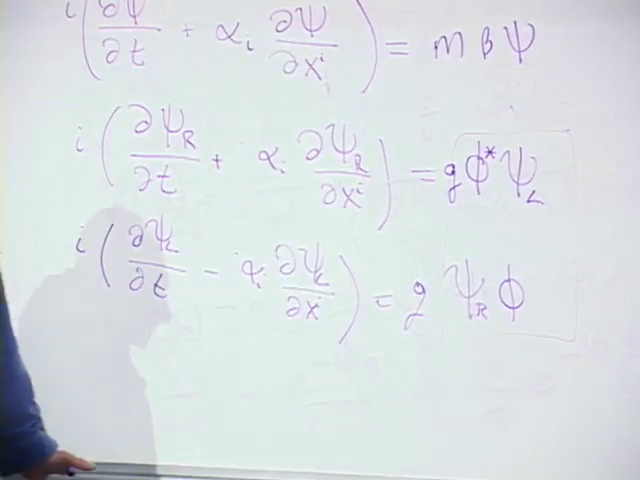
\includegraphics[width=0.76\textwidth]{lecture_09_figure_06.png}
\caption{右侧的裸质量已被带电标量场取代。黑板上的确切符号是示意性的；不变结构在\eqref{eq:l09-yukawa-lagrangian}中给出。}
\lectureframe{00:51:30}
\label{fig:l09-yukawa-board}
\end{figure}

在对称性破缺之前，这是一种相互作用而非质量。右旋费米子只有在发射或吸收平衡荷所需的标量量子时才能变成左旋费米子。系数\(y\)是汤川耦合，而不是规范荷\(g\)。

\begin{classroomqa}
\audiencequestion{直接把\(\phi\)和
\(\phi^\dagger\)放在两个方程的右侧是否合理？
\lecturetimestamp{00:51:55}}
\lecturerresponse{这之所以合理，正是因为它们的变换相位修复了不匹配。决定性的检验不是方程的视觉形式，而是相互作用
\(\bar\psi_L\phi\psi_R+\mathrm{h.c.}\)的规范不变性。}
\end{classroomqa}

\subsection{真空将相互作用转化为质量}

现在将\(\phi\)等同于希格斯场，并让它稳定在非零真空量值上。在讲座的简化归一化下，
\begin{equation}
  \phi\simeq f,
\end{equation}
所以\eqref{eq:l09-yukawa-lagrangian}包含
\begin{equation}
  \mathcal L_Y
  \supset
  -yf\,\bar\psi_L\psi_R
  -y^*f\,\bar\psi_R\psi_L .
\end{equation}
在适当时候经过无害的相位重新定义后，费米子质量为
\begin{equation}
  m_f=yf.
  \label{eq:l09-lecture-fermion-mass}
\end{equation}
这是矢量结果\(m_A=gf\)的费米子对应物。为弱规范玻色子提供纵向极化的同一个希格斯真空，也提供了连接左右费米子所需的缺失弱荷。

在正则归一化的标准模型约定下，
\begin{equation}
  H(x)=\frac1{\sqrt2}
  \begin{pmatrix}
    0\\ v+h(x)
  \end{pmatrix},
  \qquad v\simeq246\ \mathrm{GeV},
  \label{eq:l09-sm-higgs-vacuum}
\end{equation}
因此
\begin{equation}
  m_f=\frac{y_fv}{\sqrt2}.
  \label{eq:l09-sm-fermion-mass}
\end{equation}
讲座中的\(f\)与常规的\(v/\sqrt2\)仅相差这一归一化选择。

\begin{classroomqa}
\audiencequestion{如果只有乘积\(yf\)才是费米子质量，那么耦合\(y\)和真空标度\(f\)如何能分别确定？
\lecturetimestamp{00:55:36}}
\lecturerresponse{一旦规范耦合已知，弱规范玻色子质量就确定了真空标度。然后，费米子的测量质量确定其汤川耦合。在完整理论中，
\(m_W=gv/2\)、\(m_Z=v\sqrt{g^2+g'^2}/2\)和
\(y_f=\sqrt2m_f/v\)。}
\end{classroomqa}

\begin{classroomqa}
\audiencequestion{弱玻色子质量大约是\(900\ \mathrm{GeV}\)吗？
\lecturetimestamp{00:57:43}}
\lecturerresponse{不；讲座立即将这一口误更正为大约
\(90\ \mathrm{GeV}\)。更精确地说，
\(m_W\simeq80\ \mathrm{GeV}\)和\(m_Z\simeq91\ \mathrm{GeV}\)，而
底层真空标度为\(v\simeq246\ \mathrm{GeV}\)。}
\end{classroomqa}

\subsection{一个真空标度，多个汤川耦合}

每一种带电费米子都有其自身的汤川耦合：
\begin{equation}
  m_i=y_i f
  \qquad\text{(lecture normalization)}.
  \label{eq:l09-mass-family}
\end{equation}

\begin{figure}[htbp]
\centering
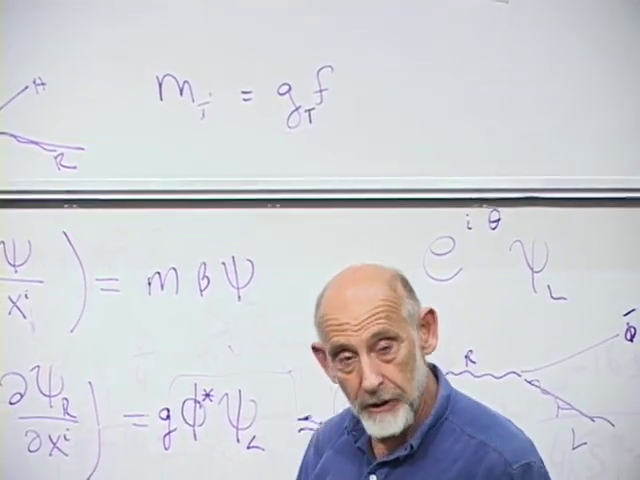
\includegraphics[width=0.76\textwidth]{lecture_09_figure_08.png}
\caption{黑板上将种类依赖性总结为\(m_i=g_i f\)；
那里写下的\(g_i\)就是此处称为\(y_i\)的汤川耦合。}
\lectureframe{01:16:30}
\label{fig:l09-mass-family-board}
\end{figure}

对于电子，讲座估计
\begin{equation}
  y_e\sim\frac{0.5\ \mathrm{MeV}}{10^2\ \mathrm{GeV}}
  \sim10^{-5}.
\end{equation}
使用正则值\(v=246\ \mathrm{GeV}\)给出更精确的
\(y_e\simeq2.9\times10^{-6}\)。顶夸克位于相反的一端：
\begin{equation}
  y_t=\frac{\sqrt2m_t}{v}\simeq1.
\end{equation}
因此，希格斯机制解释了规范不变的质量如何能够存在，但它并未解释\(y_i\)之间巨大的等级差异。观测到的费米子质量只是将该等级差异转化为测量数值。

\begin{classroomqa}
\audiencequestion{顶夸克真的具有量级为一的汤川耦合吗？\lecturetimestamp{00:59:09}}
\lecturerresponse{是的。它的质量与电弱尺度相当，因此其耦合并不像电子那样是一个微小的微扰数。在现代归一化下，\(y_t\)接近于一。}
\end{classroomqa}

\subsection{恢复物理的希格斯涨落}

将标量场冻结在其真空值上隐藏了径向激发。示意性地恢复它：
\begin{equation}
  \phi(x)\simeq f+h(x).
\end{equation}
汤川因子变为
\begin{equation}
  y\phi\simeq yf+yh=m_f+yh.
  \label{eq:l09-mass-plus-higgs}
\end{equation}

\begin{figure}[htbp]
\centering
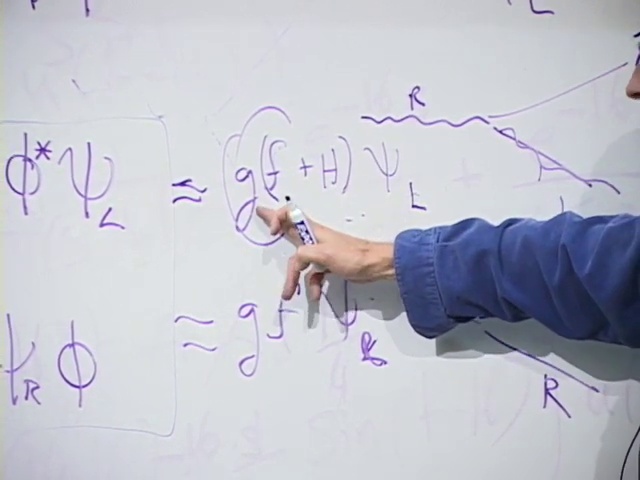
\includegraphics[width=0.76\textwidth]{lecture_09_figure_07.png}
\caption{黑板上的内容恢复了汤川项内部的希格斯涨落：常数部分产生费米子质量，涨落部分产生希格斯的发射或吸收。}
\lectureframe{01:01:15}
\label{fig:l09-higgs-fluctuation-board}
\end{figure}

\eqref{eq:l09-mass-plus-higgs}中的第一项是质量。第二项是一个顶点，其中希格斯玻色子与费米子耦合。在标准的标准模型记法中，
\begin{equation}
  \mathcal L_Y
  \supset
  -m_f\bar\psi\psi
  -\frac{m_f}{v}h\bar\psi\psi.
  \label{eq:l09-higgs-fermion-vertex}
\end{equation}
该耦合正比于费米子质量。受运动学、色因子、相空间以及竞争道的制约，希格斯因此与较重的费米子耦合更强。

\begin{classroomqa}
\audiencequestion{耦合常数本身是概率吗？\lecturetimestamp{01:03:35}}
\lecturerresponse{它们进入量子振幅。一个简单的速率往往正比于振幅的模平方，因而正比于耦合的平方，但相空间、自旋求和、干涉、圈图以及多个顶点也起作用。不应将耦合直接等同于概率。}
\end{classroomqa}

\begin{classroomqa}
\audiencequestion{这一论证是否假设只有一个希格斯场？\lecturetimestamp{01:03:59}}
\lecturerresponse{它描述的是最小标准模型，其中有一个复希格斯二重态。其四个实分量中的三个被\(W^\pm\)和\(Z\)吸收，留下一个物理的中性标量。扩展模型可以包含更多的二重态或其他标量多重态。超对称模型通常需要两个希格斯二重态，因此包含若干个物理的希格斯态。}
\end{classroomqa}

这一历史上的预期现在可以与实验相比较。
\editorialnote{本讲录制于希格斯发现之前。ATLAS和CMS于2012年宣布了一种类希格斯粒子，现在测得其质量接近\(125\ \mathrm{GeV}\)。其观测到的耦合大体上与正比于质量的标准模型模式一致。关于它优先衰变到最重粒子的说法始终带有运动学上的限制条件：一个在壳的\(t\bar t\)对对于\(125\ \mathrm{GeV}\)的希格斯来说太重了。}

\section{反粒子、束流与手征性的含义}

在转向中微子之前，课堂回到关于反粒子和加速器束流的几个操作性问题。

\begin{classroomqa}
\audiencequestion{左手电子的反粒子具有什么手性？\lecturetimestamp{01:06:05}}
\lecturerresponse{在超相对论极限下，左手征电子场湮灭左手螺旋度的电子并产生右手螺旋度的正电子。这正是必须仔细区分粒子与反粒子、手征性与螺旋度的地方之一。}
\end{classroomqa}

\begin{classroomqa}
\audiencequestion{电子和正电子能否碰撞产生一个\(Z\)玻色子？\lecturetimestamp{01:07:13}}
\lecturerresponse{能，当它们的质心能量与允许的道匹配时。电子--正电子对撞机以极高的精度研究了\(Z\)共振。整个过程中电荷和其他量子数守恒。}
\end{classroomqa}

\begin{classroomqa}
\audiencequestion{正电子都是通过某一种特殊的弱过程产生的吗？\lecturetimestamp{01:07:37}}
\lecturerresponse{不是。对产生是一种标准的电磁途径。例如，一个高能电子可以辐射出一个虚光子，而该光子可以在另一个粒子的场中产生一个\(e^-e^+\)对。本讲用费曼图对此作了示意。}
\end{classroomqa}

\begin{classroomqa}
\audiencequestion{直线加速器能否选择其电子的速度或能量？\lecturetimestamp{01:09:24}}
\lecturerresponse{能。加速场和定时选择了一个能量范围。一旦电子处于超相对论状态，其速度就已经极其接近\(c\)，因此额外的加速器能量主要增加动量和总能量，而不是明显地增加速度。}
\end{classroomqa}

\begin{classroomqa}
\audiencequestion{加速器能否制备一种极化状态的束流？\lecturetimestamp{01:09:47}}
\lecturerresponse{能，尽管这在技术上要求很高。人们可以在低能下用自旋相关的源制备自旋极化的电子，然后在控制自旋进动的同时加速它们。现代对撞机量化所得的束流极化，而不是将其视为完全纯的。}
\end{classroomqa}

\section{中微子质量与马约拉纳可能性}

\subsection{为什么中微子质量迫使人们进行扩展}

最初的最小标准模型只包含左手手性中微子场，因此预言中微子无质量。中微子振荡表明，至少有两个中微子质量本征值不同，并且中微子质量非零，尽管与带电费米子质量相比极其微小。

\begin{classroomqa}
\audiencequestion{中微子质量有多小，它们的右手分量在哪里？\lecturetimestamp{01:10:38}}
\lecturerresponse{振荡确定的是质量平方差，而不是绝对质量。相关的劈裂对应大约\(0.009\ \mathrm{eV}\)和\(0.05\ \mathrm{eV}\)的尺度。狄拉克描述添加惰性右手手性中微子；马约拉纳描述则把缺失的手性联系到电荷共轭中微子场。}
\end{classroomqa}

对于狄拉克中微子，人们添加一个新场\(\nu_R\)，并重复汤川构造：
\begin{equation}
  \mathcal L_{\nu,\mathrm{Dirac}}
  =-y_\nu\bar L\,\widetilde H\,\nu_R+\mathrm{h.c.},
  \qquad
  m_\nu=\frac{y_\nu v}{\sqrt2}.
  \label{eq:l09-dirac-neutrino}
\end{equation}
所需的\(y_\nu\)极其微小。

还有另一种逻辑可能性，因为中微子不带电荷。左手手性中微子可以与其自身的电荷共轭耦合，而后者具有相反的手性：
\begin{equation}
  \nu_L\longleftrightarrow(\nu_L)^c_R .
  \label{eq:l09-majorana-mixing}
\end{equation}
以这种方式构建的质量本征态是马约拉纳费米子：在相位约定下，它就是自身的反粒子。类似的电子--正电子混合被禁止，因为这会违反严格的电荷守恒。

\begin{classroomqa}
\audiencequestion{为什么粒子--反粒子混合对中微子允许，而对电子不允许？\lecturetimestamp{01:13:43}}
\lecturerresponse{电子和正电子具有相反的电荷，因此将它们作为同一个单粒子态混合的质量项会违反未破缺的电磁对称性。中微子电中性。如果没有严格的守恒轻子数将其与反粒子区分开来，马约拉纳质量就是允许的。}
\end{classroomqa}

这一名称是为了纪念埃托雷·马约拉纳，这位年轻的意大利物理学家提出了这种实费米子表示，并于1938失踪。讲座在此停顿于这一历史谜团：他的命运从未被确定。
\editorialnote{对于标准模型中的活跃中微子，规范不变的马约拉纳质量在电弱破缺之前并不是可重整的裸质量项。在低能下，它可以来自五维温伯格算符\((LH)(LH)/\Lambda\)，或者通过涉及重惰性中微子的跷跷板机制产生。中微子是狄拉克粒子还是马约拉纳粒子，在实验上仍未确定。}

\section{为什么熟悉的谱系聚集在电弱能标附近}

\subsection{共同能标及其重要限定}

\begin{classroomqa}
\audiencequestion{为什么曾预期希格斯质量可在弱能标处达到？\lecturetimestamp{01:14:48}}
\lecturerresponse{希格斯势的曲率决定径向希格斯质量，而同一个真空能标\(f\)决定\(W\)和\(Z\)的质量。因此，如果没有极端的标量自耦合，人们预期希格斯质量与弱能标处于同一宽泛量级。观测到的\(125\ \mathrm{GeV}\)值确实位于那里。}
\end{classroomqa}

讲座引人注目的总结是，最小标准模型的基本质量都可追溯到一个破缺的真空：
\begin{align}
  m_W&=\frac12gv,\\
  m_Z&=\frac12\sqrt{g^2+g'^2}\,v,\\
  m_f&=\frac1{\sqrt2}y_fv.
  \label{eq:l09-electroweak-mass-summary}
\end{align}
如果\(v\)消失而无量纲耦合保持不变，那么弱规范玻色子和带电基本费米子都将无质量。

这一陈述不得超出其适用范围。光子和胶子仍然无质量，因为未破缺的规范对称性保护它们。质子和中子的大部分质量是QCD束缚能，而不是其夸克希格斯质量之和。中微子质量需要扩展最小模型。希格斯质量本身取决于标量势，并不只是另一个汤川质量。

\subsection{质量不必等待对称性破缺的粒子}

假设一种新费米子具有规范量子数相同的左手和右手手性分量。那么
\(\bar\Psi_L\Psi_R+\mathrm{h.c.}\)已经是规范不变的。这样的\emph{矢量型}费米子可以拥有与\(v\)无关的裸质量\(M\)：
\begin{equation}
  \mathcal L_{\mathrm{vectorlike}}
  =-M\bar\Psi\Psi.
  \label{eq:l09-vectorlike-mass}
\end{equation}
对于\(M\gg v\)，不存在电弱对称性障碍。

这引出了讲座关于自然性的宽泛论证。受规范对称性或手性对称性保护的粒子保持无质量，直到希格斯真空破坏该保护，因此它们的质量与相对较小的能标\(v\)相联系。没有这种保护的粒子可能自然重得多，因而从观测到的低能谱中缺席。我们所看到的可能是一种选择效应：可及的粒子正是那些其质量被迫等待电弱对称性破缺的粒子。

\begin{classroomqa}
\audiencequestion{具有独立且大得多的质量的粒子在现实中是否不起任何作用？\lecturetimestamp{01:19:39}}
\lecturerresponse{它们在普通的低能实验室物理中作用很小，因为难以产生，但它们仍可能塑造高能历史或宇宙学。讲座提出暗物质作为一个可能场所，在那里较重的隐藏谱也许首先显露自身。}
\end{classroomqa}

2010年的讨论反映了当时流行的对弱尺度或稍重暗物质的预期。那仍然是一类有用的模型，而非已确立的事实。暗物质已通过引力被探测到，但其粒子身份及其质量起源仍然未知。

\section{结束提问：宇宙射线、惯性、引力与手征性}

\subsection{质量不等于高实验室能量}

\begin{classroomqa}
\audiencequestion{宇宙射线的质量是多少？
\lecturetimestamp{01:20:57}}
\lecturerresponse{宇宙射线可以是质子、原子核、电子或光子；其不变质量就是该粒子或系统的质量。引人注目的是其实验室能量，对于最高能事件，该能量大致达到\(10^{20}\)至\(10^{21}\ \mathrm{eV}\)。高能量并不等同于高不变质量。}
\end{classroomqa}

宇宙射线撞击一个近似静止的靶粒子。对于实验室能量为\(E\gg m_p\)的入射质子，
\begin{equation}
  s=(p_1+p_2)^2
  \simeq2m_pE+2m_p^2,
  \qquad
  \sqrt{s}\simeq\sqrt{2m_pE}.
  \label{eq:l09-fixed-target-s}
\end{equation}
只有入射能量的平方根成为质心能量。对于能量为\(E_{\rm beam}\)的等能对撞束，
\begin{equation}
  \sqrt{s}\simeq2E_{\rm beam}.
  \label{eq:l09-collider-s}
\end{equation}
这就是为什么在将受控束能量转化为新粒子质量方面，对撞机远比固定靶高效。

\begin{classroomqa}
\audiencequestion{为什么CERN的对撞机可以比单个能量高得多的粒子撞击静止物质成为更有力的探针？
\lecturetimestamp{01:21:50}}
\lecturerresponse{在固定靶碰撞中，动量守恒使大部分实验室能量以末态运动的形式向前带走。在对称对撞机中，总空间动量可以为零，从而使束能量可作为质心能量使用。能量最高的宇宙射线在\(\sqrt{s}\)方面仍可超过LHC，但它们到达不可预测，且不能提供对撞机光度或受控的探测器环境。}
\end{classroomqa}

\subsection{静止质量与对加速度的抵抗}

\begin{classroomqa}
\audiencequestion{惯性与质量本质上是同一回事吗？
\lecturetimestamp{01:22:41}}
\lecturerresponse{在静止时，不变质量既通过\(E_0=mc^2\)成为静止能量，又是支配低速下对力响应的参数。狭义相对论解释了为什么这些定义属于同一个量。对于运动物体，更清楚的做法是保持不变质量固定，并用相对论能量和动量描述加速度。}
\end{classroomqa}

不变关系
\begin{equation}
  E^2=p^2c^2+m^2c^4
  \label{eq:l09-energy-momentum}
\end{equation}
包含这两种含义。在静止附近，
\begin{equation}
  E=mc^2+\frac{p^2}{2m}+\cdots,
\end{equation}
因此给出静止能量的同一个\(m\)也出现在动能响应中。在高速下，力与加速度之间的关系取决于力是平行还是垂直于速度。这种方向依赖性正是现代处理避免依赖速度的\emph{相对论质量}、并将质量保留给洛伦兹不变量\(m\)的原因。

\subsection{引力与什么耦合}

\begin{classroomqa}
\audiencequestion{一旦希格斯赋予粒子质量，它是否就开始与引力耦合？
\lecturetimestamp{01:23:58}}
\lecturerresponse{其静止能量对引力有贡献，但质量并非全部来源。光子无质量，却仍被引力偏折。在广义相对论中，来源是应力--能量张量：能量密度、动量流、压强和应力。对于缓慢运动的物质，主导贡献是其静止质量能量。}
\end{classroomqa}

太阳附近的光线弯曲在操作层面说明了这一点。光子尽管具有\(m=0\)，仍响应时空曲率，而且其能量和动量也对引力场有贡献。对于两个近乎静止的大质量物体，能量由\(mc^2\)主导，因此牛顿引力可以用它们的质量写出，而不必展示更一般的应力--能量表述。

\begin{classroomqa}
\audiencequestion{高能粒子在每个方向上是否都同样更难被加速？
\lecturetimestamp{01:25:20}}
\lecturerresponse{不是。平行于运动的力所引起的动量变化不同于横向力所引起的变化。能量更高的粒子确实更难被偏转，但赋予它一个增大的运动质量会掩盖这种方向结构。}
\end{classroomqa}

\subsection{静止电子与所承诺的区分}

\begin{classroomqa}
\audiencequestion{静止的电子怎么能被称为左旋或右旋？\lecturetimestamp{01:26:32}}
\lecturerresponse{静止时无法赋予它螺旋度，因为螺旋度要用动量的方向。静止的自旋量仍然可以分解为左手征分量和右手征分量。对于有质量的电子，两个分量都存在，而质量项将它们耦合起来。}
\end{classroomqa}

\begin{classroomqa}
\audiencequestion{如果静止的电子没有螺旋度，它还能参与弱相互作用吗？\lecturetimestamp{01:27:18}}
\lecturerresponse{能。弱相互作用耦合到手征，而不是耦合到依赖于参考系的螺旋度标签。在高能下，螺旋度是手征的方便近似；在接近静止时，这种捷径失效。这就是讲座此前推迟讨论的微妙区别。}
\end{classroomqa}

\section{历史性的课后问题}

\subsection{发现之前的希格斯窗口}

在2010年，希格斯尚未被观测到。精确电弱观测量，尤其是\(W\)、\(Z\)、顶夸克及其他参数之间对圈图敏感的关系，在标准模型内倾向于一个相对较轻的希格斯。讲座引用了一个可能的上限区域，接近\(160\ \mathrm{GeV}\)，远低于\(v\)，但并未相差一个数量级。

\begin{classroomqa}
\audiencequestion{当时有什么证据表明希格斯比\(250\ \mathrm{GeV}\)真空标度更轻？\lecturetimestamp{01:28:28}}
\lecturerresponse{高精度测量可以与辐射修正相比较，而后者的数值对数依赖于希格斯质量。由此得到的全局拟合倾向于一个轻希格斯。这是间接证据，不是直接的质量测量；后来的直接数值约为\(125\ \mathrm{GeV}\)。}
\end{classroomqa}

\begin{classroomqa}
\audiencequestion{希格斯势的多个极小值能否产生不同的\(f\)值，也许与不同的粒子世代有关？\lecturetimestamp{01:29:28}}
\lecturerresponse{不同的极小值可以支撑非常不同的低能物理，但从观测到的世代并不能简单推断出多个希格斯极小值。讲座将多重真空这一更广泛的主题推迟到后续课程，而不是假装在这里解决它。}
\end{classroomqa}

\begin{classroomqa}
\audiencequestion{希格斯是否被预期为在LHC发现的第一种新粒子？\lecturetimestamp{01:31:32}}
\lecturerresponse{不一定。它的可见性取决于产生率和衰变道，其中一些可能难以观测或不可见。在LHC数据之前，超对称粒子或其他新粒子有可能先出现。历史上，希格斯被发现了，而尚未确立任何超对称粒子。}
\end{classroomqa}

\subsection{当一个中性粒子是它自己的反粒子时}

\begin{classroomqa}
\audiencequestion{光子和胶子没有反粒子是因为它们无质量吗？\lecturetimestamp{01:32:12}}
\lecturerresponse{不是。无质量并不是判据。光子是它自己的反粒子，因为没有守恒荷区分光子和反光子。每个胶子在适当的色表示中也是自共轭的规范量子，尽管胶子本身带色，而且色标签在电荷共轭下会混合。中子电中性，但有一个不同的反中子，因为重子数及其夸克组分将它们区分开来。}
\end{classroomqa}

中微子作为微妙的情形回归。它有弱相互作用，而被称为中微子和反中微子的超相对论态以相反的螺旋度相互作用。如果某个精确的轻子数将它们区分开来，它们可以形成一个带有不同反粒子的狄拉克粒子。如果轻子数不精确，而质量是马约拉纳型的，那么有质量粒子就是它自己的反粒子，尽管它的两个螺旋度态在弱过程中行为不同。

\begin{classroomqa}
\audiencequestion{弱荷和轻子数能证明中微子和反中微子必然不同吗？\lecturetimestamp{01:32:46}}
\lecturerresponse{不能确凿地证明。弱相互作用区分螺旋度态，但马约拉纳质量可以将中微子场与其电荷共轭组合起来。决定性问题在于，是否存在一个精确守恒的量子数禁止这种混合。标准模型并未将总轻子数作为精确的规范对称性强加。}
\end{classroomqa}

普通味振荡需要另作提醒。\editorialnote{普通观测到的味振荡混合的是同一中微子或反中微子扇区内的\(\nu_e,\nu_\mu,\nu_\tau\)；它们本身并不证明中微子--反中微子的转化。诸如无中微子双贝塔衰变之类的破坏轻子数过程将为马约拉纳质量提供直接证据，但迄今尚未确认任何此类过程。}

\begin{classroomqa}
\audiencequestion{标准模型是否解释了电荷为何是量子化的？\lecturetimestamp{01:33:39}}
\lecturerresponse{讲座承认了这个问题，但并未展开。在标准模型内部，规范不变性与反常相消对自洽的超荷赋值施加了很强的限制；更深入的解释往往要诉诸大统一或其他紫外结构。}
\end{classroomqa}

\section{讲座已经确立的内容}

规范玻色子与费米子的故事现在彼此吻合了。

\begin{enumerate}
  \item 仅含导数的规范理论对于均匀矢量势不存在能隙。规范对称性禁止裸矢量质量。
  \item 具有非零真空量值的带电标量贡献
  \(g^2f^2A_\mu A^\mu\)。它的角向戈德斯通模成为有质量弱规范玻色子的纵向极化。
  \item 狄拉克质量将\(\psi_L\)与\(\psi_R\)耦合起来。由于弱相互作用赋予二者不同的规范量子数，裸的左--右质量项是被禁止的。
  \item 汤川相互作用将希格斯场插入两种手征性之间，并且是规范不变的。将希格斯场替换为其真空值给出\(m_f=y_ff\)，而保留其涨落则给出物理的希格斯--费米子耦合。
  \item 中微子质量遵循同样的左--右逻辑，但由于中微子电中性，它同时允许狄拉克实现与马约拉纳实现。
  \item 没有规范保护或手征保护的粒子可以拥有与电弱能标无关的质量，并且可能远高于当前实验所能触及的范围。
\end{enumerate}

因此，统一的陈述并不是说希格斯是一种机械地拖拽粒子的物质。而是说电弱真空具有非零的标量序参量。该序参量改变了低能方程中哪些规范不变项是可能的。对于矢量，它打开了一个零动量能隙；对于费米子，它允许左--右混合。不同的质量于是度量了与同一个破缺真空的不同耦合。